\documentclass[tikz, border=5mm]{standalone}
\usetikzlibrary{arrows.meta}
\definecolor{ovalcolor}{RGB}{180,180,180}
\colorlet{myred}{red!80!black}
\colorlet{myblue}{blue!80!black}
\colorlet{mybluee}{myblue!80!black}
\colorlet{mygreen}{green!60!black}
\colorlet{mydarkred}{red!30!black}
\colorlet{mydarkblue}{blue!40!black}
\colorlet{mydarkgreen}{green!30!black}

\begin{document}
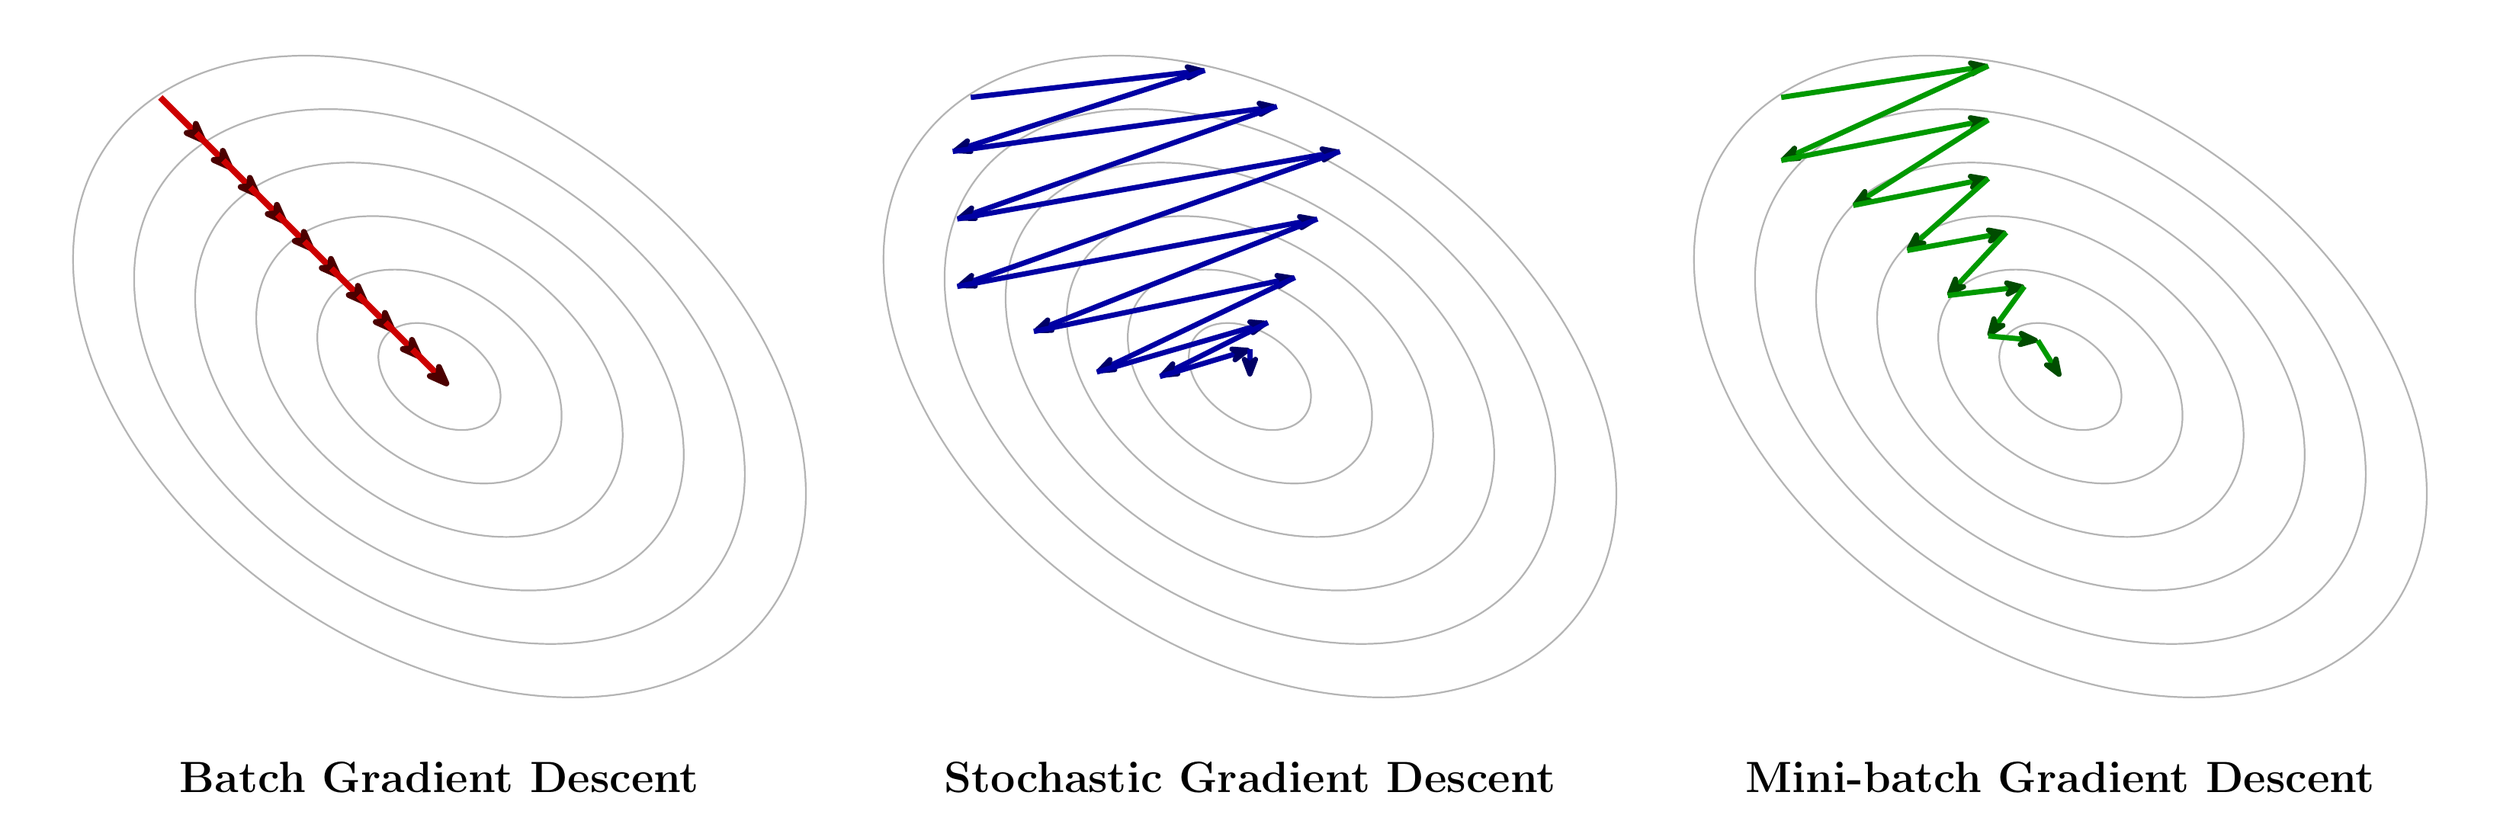
\begin{tikzpicture}[>=stealth, scale=0.75,
    barr/.style={line width=3pt,   myred,   -{Stealth[round,color=mydarkred]}},
    sarr/.style={line width=2.5pt, mybluee, -{Stealth[round,color=mydarkblue]}},
    marr/.style={line width=2.5pt, mygreen, -{Stealth[round,color=mydarkgreen]}}]

  % ---- 三组等高线椭圆（中心分别在 -6 / 12 / 30）----
  \foreach \x in {-6,12,30}{
    \begin{scope}[shift={(\x,0)}]
      \foreach \r in {1,...,6}
        \draw[ovalcolor, thick, rotate=145] (0,0) ellipse ({\r*1.5} and {\r});
    \end{scope}
  }

  % ---- 标题 ----
  \node at (-6,-8.9) {\huge\textbf{Batch Gradient Descent}};
  \node at (12,-8.9) {\huge\textbf{Stochastic Gradient Descent}};
  \node at (30,-8.9) {\huge\textbf{Mini-batch Gradient Descent}};

  % ---- Batch：方向稳定，笔直指向中心 ----
  \draw[barr] (-12.2,6.2) -- (-11.2,5.2);
  \draw[barr] (-11.4,5.4) -- (-10.6,4.6);
  \draw[barr] (-10.8,4.8) -- (-10.0,4.0);
  \draw[barr] (-10.2,4.2) -- (-9.4,3.4);
  \draw[barr] (-9.6,3.6)  -- (-8.8,2.8);
  \draw[barr] (-9.0,3.0)  -- (-8.2,2.2);
  \draw[barr] (-8.4,2.4)  -- (-7.6,1.6);
  \draw[barr] (-7.8,1.8)  -- (-7.0,1.0);
  \draw[barr] (-7.2,1.2)  -- (-6.4,0.4);
  \draw[barr] (-6.6,0.6)  -- (-5.8,-0.2);
  
  % ---- SGD：整体左移、高处右甩收进椭圆内，收敛到中心 ----
  \draw[sarr] (5.8,6.2)  -- (11.0,6.8);
  \draw[sarr] (11.0,6.8) -- (5.4,5.0);
  \draw[sarr] (5.4,5.0)  -- (12.6,6.0);
  \draw[sarr] (12.6,6.0) -- (5.5,3.5);
  \draw[sarr] (5.5,3.5)  -- (14.0,5.0);
  \draw[sarr] (14.0,5.0) -- (5.5,2.0);
  \draw[sarr] (5.5,2.0)  -- (13.5,3.5);
  \draw[sarr] (13.5,3.5) -- (7.2,1.0);
  \draw[sarr] (7.2,1.0)  -- (13.0,2.2);
  \draw[sarr] (13.0,2.2) -- (8.6,0.1);
  \draw[sarr] (8.6,0.1)  -- (12.4,1.2);
  \draw[sarr] (12.4,1.2) -- (10.0,0.0);
  \draw[sarr] (10.0,0.0) -- (12.0,0.6);
  \draw[sarr] (12.0,0.6)-- (12,0);

  % ---- Mini-batch：同样左收，幅度比 SGD 小，收敛到中心 ----
  \draw[marr] (23.8,6.2) -- (28.4,6.9);
  \draw[marr] (28.4,6.9) -- (23.8,4.8);
  \draw[marr] (23.8,4.8) -- (28.4,5.7);
  \draw[marr] (28.4,5.7) -- (25.4,3.8);
  \draw[marr] (25.4,3.8) -- (28.4,4.4);
  \draw[marr] (28.4,4.4) -- (26.6,2.8);
  \draw[marr] (26.6,2.8) -- (28.8,3.2);
  \draw[marr] (28.8,3.2) -- (27.5,1.8);
  \draw[marr] (27.5,1.8) -- (29.2,2.0);
  \draw[marr] (29.2,2.0) -- (28.4,0.9);
  \draw[marr] (28.4,0.9) -- (29.5,0.8);
  \draw[marr] (29.5,0.8) -- (30,0);

\end{tikzpicture}
\end{document}